\chapter{Generative models}

\section{Variational Autoencoders}
Generative modeling is an area of machine learning that deals with models of distributions $p(x)$, defined over datapoints $x$ in some potentially high-dimensional space $\mathcal{X}$. 
Unlike the previous autoencoder model, here we do not aim to learn a compact representation of the input and then reconstruct it. Instead, we want to learn the probability distribution of the data, that is, the probability of each element in the dataset.

There are two main reasons for doing this:
\begin{compactitemize}
    \item \textbf{Sampling}: if we know the data distribution, we can sample from it to generate new data.
    \item \textbf{Anomaly Detection}: after training, we can evaluate the probability of a given datapoint under the learned distribution. If the probability is high, we can consider the datapoint as "normal"; if it is low, the datapoint is likely to be different in some way, and thus considered anomalous.
\end{compactitemize}

\subsection{The problem of the distribution and the Latent Variables}
\begin{wrapfigure}{r}{0.25\textwidth}
    \centering
    \vspace{-10pt}
    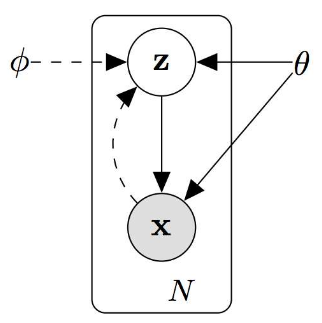
\includegraphics[width=\linewidth]{images/latent_variable_model.png}
    \label{fig:Scaled Dot Product Attention}
    \vspace{-10pt}
\end{wrapfigure}
Typically, we work with complex data (e.g., images), so using a very simple distribution (such as a normal distribution) to represent our data can be inefficient.
Taking a step back, denoising autoencoders and contractive autoencoders implicitly learn the structure of the probability distribution p(x), but sampling new examples from these models is very complex because the learned distribution is encoded implicitly in the network weights and there is no defined sampling mechanism.
Therefore, we would ideally like to have a distribution $p(x)$ that is simple enough to allow efficient sampling, yet expressive enough to represent our data in a realistic way. The key idea is to map our data into another space where a simple distribution is sufficient, and then map samples drawn from this simple distribution back to the original data space. 
This concept is known as \textbf{Latent Variable Models}. Essentially, we model the probability of the observable data based on some underlying variables (called latent variables) that are not directly observable. These latent variables capture hidden characteristics of the data and allow us to describe complex distributions using simpler ones.

\subsection{Latent Variables in Weather Modeling}
\begin{wrapfigure}{r}{0.3\textwidth}
    \centering
    \vspace{-10pt}
    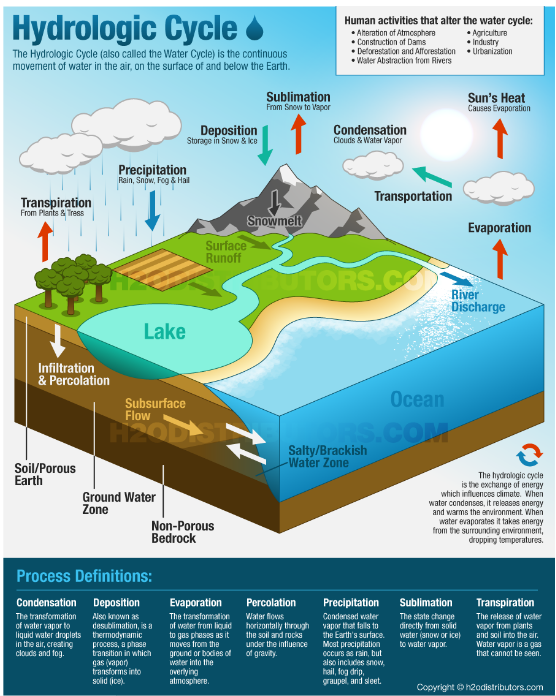
\includegraphics[width=\linewidth]{images/WM.png}
    \label{fig:Scaled Dot Product Attention}
    \vspace{-10pt}
\end{wrapfigure}
The idea in this examples is that latent variables can represent hidden physical quantities that exaplain observable data.
We can measure quantities like temperature, humidity, and wind speed. However, these depend on other \textbf{unobserved pysical factors} like:
\begin{compactitemize}
    \item pressure gradients in the atmosphere
    \item altitude temperature profiles
    \item vapor concentration and cloud density
\end{compactitemize}
These hidden quantities form the \textbf{latent variables} $z$.
They govern the observable weather data $x$, even if we cannot measure them directly.


\subsection{Latent Variable Models}
Latent Variable Models relate a set of \textbf{observable} variables $x$ to a set of \textbf{latent} (hidden) variables $z$.  
The latent variables represent underlying factors that are not directly observable, but that influence the formation of the data.

We assume that the data $x$ is generated from some latent variable $z$, therefore:
\[
p(x, z) = p(x \mid z)\, p(z),
\]
where:
\begin{itemize}
    \item $p(z)$ is the \textbf{prior distribution} of the latent variables (typically chosen to be simple, e.g., a Gaussian),
    \item $p(x \mid z)$ is the \textbf{generative model}, describing how data $x$ is generated from $z$.
\end{itemize}

Since $z$ is not observed, the probability distribution of the observable data $x$ is obtained by \textbf{marginalizing} over $z$:
\[
p(x) = \int p(x, z)\, dz = \int p(x \mid z)\, p(z)\, dz.
\]

This follows from:
\begin{itemize}
    \item \textbf{Law of Total Probability}: $\displaystyle p(x) = \int p(x, z)\, dz$,
    \item \textbf{Definition of Conditional Probability}: $\displaystyle p(x, z) = p(x \mid z)\, p(z)$.
\end{itemize}

The integral
\[
p(x) = \int p(x \mid z)\, p(z)\, dz
\]
is often \textbf{intractable} in closed form, especially when $z$ has high dimensionality or the model is complex.  
This is one of the central challenges in Bayesian statistics and probabilistic machine learning.

A practical way to approximate $p(x)$ is through Monte Carlo sampling:
\[
p(x) \approx \frac{1}{K} \sum_{k=1}^{K} p(x \mid z^{(k)}), \qquad z^{(k)} \sim p(z).
\]

The sampling procedure is:
\begin{enumerate}
    \item Sample a latent variable: $z \sim p(z)$,
    \item Generate an observation: $x \sim p(x \mid z)$.
    \item Apply Monte Carlo approximation $z \rightarrow x.$
\end{enumerate}

\subsection{Problem with Monte Carlo}
The monte carlo approximation heavly depends of which sample has been sampled by $p(z)$, and we need a large number of sample to get a good estimate of $p(x)$ and most of $z$'s sampled are irrelevant for the specific observation of $x$.

The idea to solve this problem is learn a model that, given an observation $x$, predicts the most \textbf{plausible latent variables} $z$, those that are \textbf{more likely related} to $x$ under the true posterior distribution $p(z|x)$.

\subsection{Variational Inference}

Variational Inference is a framework used to approximate intractable posterior distributions.  
The central idea is to replace the true posterior distribution $p(z \mid x)$, which is often complex and computationally expensive, with a simpler and tractable distribution $q(z \mid x)$, called the \textbf{Proposal distribution} or \textbf{approximate posterior}.

The goal is to choose a family of distributions $q(z \mid x)$ that is:
\begin{compactitemize}
    \item expressive enough to approximate $p(z \mid x)$ well,
    \item but simple enough to evaluate and to sample from efficiently.
\end{compactitemize}

This allows us to approximate integrals of the form:
\[
p(x) = \int p(x \mid z)\, p(z)\, dz,
\]
using a small number of meaningful samples drawn from $q(z \mid x)$ rather than from $p(z)$.

The objective of variational inference is therefore to find (or learn) the approximate posterior:
\[
q^\ast(z \mid x) \approx p(z \mid x).
\]

A common way to define this objective is to minimize the Kullback–Leibler divergence between the two distributions:
\[
q^\ast(z \mid x)
= \arg\min_{q} \, D_{\mathrm{KL}}\bigl(q(z \mid x)\, \Vert\, p(z \mid x)\bigr).
\]

However, directly minimizing this divergence requires evaluating $\log p(x)$, which is generally \textbf{intractable} for complex generative models.  
This motivates the introduction of the \textbf{Evidence Lower Bound (ELBO)}, which provides a computable objective that indirectly minimizes the KL divergence.

Start with tha calulus:
\begin{align}
    q^*(z \mid x) 
    &= \arg\min_q \, D_{\mathrm{KL}}\!\left[q(z \mid x) \;\Vert\; p(z \mid x)\right] \\
    &= \mathbb{E}_{z \sim q(z \mid x)} \left[ \log q(z \mid x) - \log p(z \mid x) \right] \\
    &= \mathbb{E}_{z \sim q(z \mid x)} \left[ \log q(z \mid x) - \log \frac{p(x \mid z)\, p(z)}{p(x)} \right] \\
    &= \mathbb{E}_{z \sim q(z \mid x)} \left[ \log q(z \mid x) - \log p(x \mid z) - \log p(z) + \log p(x)\right] \\
    &= \mathbb{E}_{z \sim q(z \mid x)} \left[ \log q(z \mid x) - \log p(x \mid z) - \log p(z)\right] + \log p(x) \\
    &= \mathbb{E}_{z \sim q(z \mid x)} \left[ \log q(z \mid x) - \log p(z)\right] - \mathbb{E}_{z \sim q(z \mid x)} \left[\log p(x \mid z)\right] + \log p(x) \\
    &= D_{\mathrm{KL}} \left[q(z \mid x) \mid \mid p(z)\right] - \mathbb{E}_{z \sim q(z \mid x)} \left[\log p(x \mid z)\right] + \log p(x)
\end{align}
The equation can be written like this:
\[
\log p(x) - \color{blue} D_{\mathrm{KL}} \big[q(z \mid x) \, \Vert \, p(z \mid x)\big]
\color{black}=
\color{red}{\mathbb{E}_{z \sim q(z \mid x)}[\log p(x \mid z)] - D_{\mathrm{KL}} \big[q(z \mid x) \, \Vert \, p(z)\big]}
\]
Where:
\begin{compactitemize}
    \item the part in red is the \textbf{ELBO}, that is something that can we optimize using the  stochastic gradient descent given the right choice of $q()$.
    \item the part in blue is allways positive and is the KL divergence between the proxy and the real posterior distributions.
\end{compactitemize}

\begin{infobox}[Note]
    The equation above is important beacuse provides a relationship between $p(x)$ and the posterior distribution $q(z|x)$
\end{infobox}

So now we can write the equation like this:
\[
\log p(x) = D_{\mathrm{KL}} \big[q(z \mid x) \, \Vert \, p(z \mid x)\big] + \mathrm{ELBO}
\]
Since the $D_{KL}$ term is always non-negative, this leads to the following inequality:
\[
\log p(x) \ge \mathrm{ELBO}, \quad \text{where} \quad 
\mathrm{ELBO} = \mathbb{E}_{z \sim q(z \mid x)}[\log p(x \mid z)] 
- D_{\mathrm{KL}} \big[q(z \mid x) \, \Vert \, p(z)\big]
\]
\begin{wrapfigure}{r}{0.45\textwidth}
    \centering
    \vspace{-10pt}
    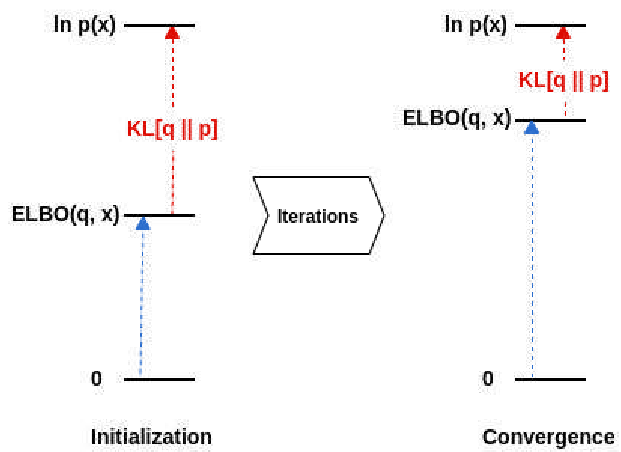
\includegraphics[width=\linewidth]{images/ELBO.png}
    \label{fig:Scaled Dot Product Attention}
    \vspace{-10pt}
\end{wrapfigure}
Results:
\begin{compactitemize}
    \item Maximizing the ELBO provides a lower bound on the true log-likelihood $\log p(x)$.
    \item Therefore, maximizing the ELBO is equivalent to making our model as close as possible to the true data distribution.
    \item If we maximize the ELBO, we simultaneously minimize the KL divergence between the true intractable posterior and the proposal/posterior (our initial goal).
\end{compactitemize}

\subsection{Variational Autoencoder: the Encoder and the Decoder}
A Variational Autoencoder (VAE) is an autoencoder trained to maximize the \textbf{Evidence Lower Bound (ELBO)}:

\[
\mathrm{ELBO} = \underbrace{\mathbb{E}_{z \sim q_\phi(z \mid x)}[\log p_\theta(x \mid z)]}_{\text{Reconstruction Term}}
- \underbrace{D_{\mathrm{KL}}\big[q_\phi(z \mid x) \, \Vert \, p(z)\big]}_{\text{Regularization Term}}
\]
\textbf{Components of the VAE:}
\begin{itemize}
    \item \textbf{Encoder network} $q_\phi(z \mid x)$: given an input $x$, it outputs a distribution (typically Gaussian) that approximates the true posterior $p(z \mid x)$.
    \begin{compactitemize}
        \item Unlike a standard autoencoder, the encoder does not output a deterministic vector, but the parameters (mean and variance) of a latent distribution.
        \item Formally: $x \to f_{\text{ENC}}(x; \phi) = [\mu(x), \sigma^2(x)]$, such that $z \sim \mathcal{N}(\mu(x), \sigma^2(x))$.
        \item In practice, the encoder outputs two vectors, $\mu(x)$ and $\sigma^2(x)$, representing the mean and variance of the approximate posterior.
    \end{compactitemize}
    \item \textbf{Decoder network} $p_\theta(x \mid z)$: reconstructs the input $x$ from a sampled latent variable $z$, modeling the likelihood of the data.
    \begin{compactitemize}
        \item The decoder takes a latent variable $z$ sampled from the encoder $q(z \mid x)$ and produces a reconstruction $x_{\text{recon}}$.
        \item Formally: $x_{\text{recon}} \to g_{\text{DEC}}(z; \theta)$, where $z \sim \mathcal{N}(\mu(x), \sigma^2(x))$.
        \item The decoder aims to maximize the conditional log-likelihood $\log p(x \mid z)$.
        \item In practice, for continuous data, this is often implemented by minimizing the Mean Squared Error (MSE) between the original input $x$ and the reconstruction $x_{\text{recon}}$.
    \end{compactitemize}    
\end{itemize}

Now take a look at the \textbf{regularization term}: we say that
\begin{compactitemize}
    \item $D_{\mathrm{KL}}[q(z \mid x) \, \Vert \, p(z)]$ is a measure of how $q(z \mid x)$ diverges from the distribution $p(z)$, called the \emph{prior distribution}.  
    \item $p(z)$ is the expected probability distribution over the latent variable; it is hand-crafted and typically follows a standard Gaussian distribution.  
    \item If both posterior and prior distributions have Gaussian form (as holds in this case), the $D_{\mathrm{KL}}$ has a closed-form equation.
\end{compactitemize}

\begin{figure}[H]
    \centering
    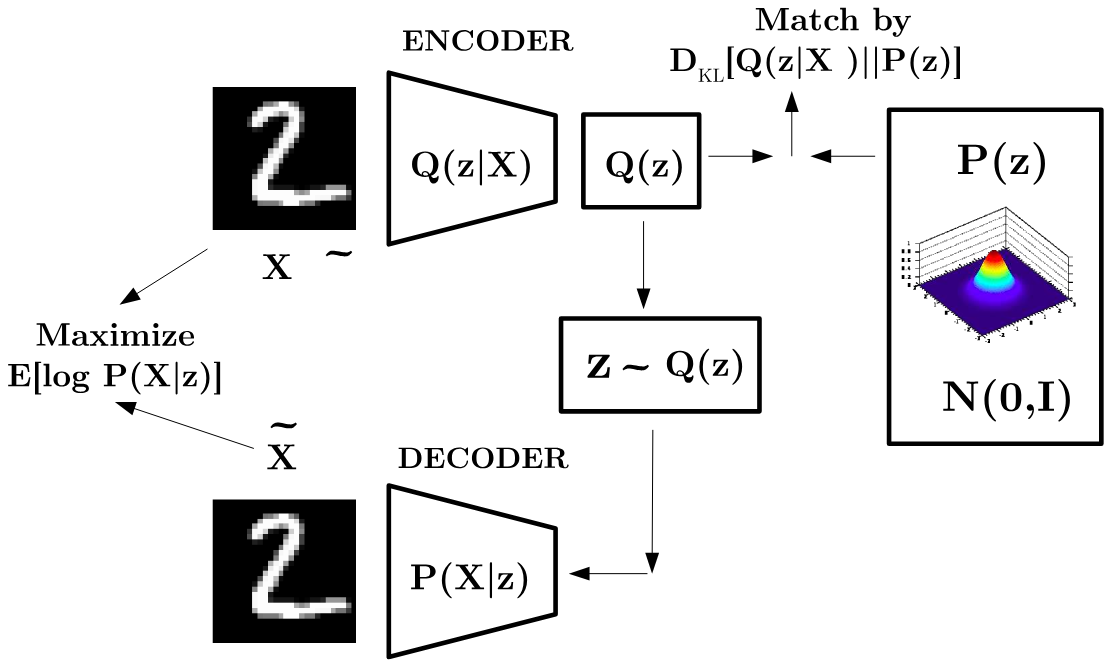
\includegraphics[width=0.5\textwidth]{images/VAE.png}
    \caption{Variational Autoencoders: overall architecture}
    \label{fig:MHA2}
\end{figure}

\subsection{The reparametrization trick}
\begin{wrapfigure}{r}{0.4\textwidth}
    \centering
    \vspace{-10pt}
    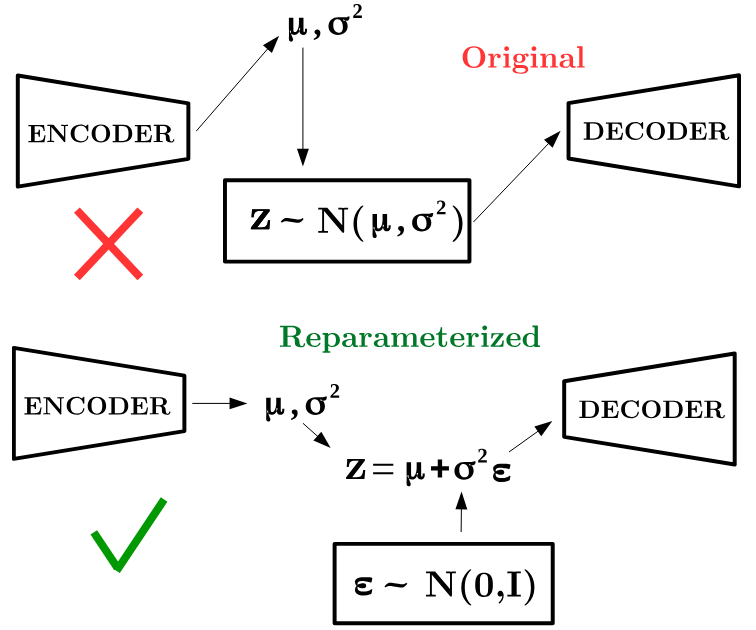
\includegraphics[width=\linewidth]{images/RP.png}
    \label{fig:Scaled Dot Product Attention}
    \vspace{-10pt}
\end{wrapfigure}
The sampling step $z \sim N(z \mid \mu(x), \sigma^2(x))$ is not differentiable, so we can not use the backpropagation to train the model.
The \textbf[reparametrize trick] lets us backpropagate through the sampling operation (a random operator). So instead of do $z \sim N(z \mid \mu(x), \sigma^2(x))$  we compute this:
\begin{compactitemize}
    \item Sample a random vector from the standard distribution $\epsilon \sim N(z \mid 0, I_n)$
    \item \textbf{Reparametrize}: $z= \mu(x) + \epsilon * \sigma(x)$
\end{compactitemize}
The advantage is that the sampled noise vector $\epsilon$ is just an extra input to the network. Its distribution is not a function of any of the variables whose derivatives we want to calculate, which allows gradients to flow through the network during backpropagation.

\section{Generative Adversarial Networks}